\subsection{Visitor}
\label{visitor}

\textbf{Scopo}: Comportamentale \\
\textbf{Raggio d'azione}: Oggetti

\paragraph{Definizione} Il pattern rappresenta un’operazione da eseguire sugli oggetti di una struttura e consente di definire nuove operazioni senza modificare le classi degli oggetti su cui opera (vantaggioso).

\paragraph{Motivazione} Un compilatore che rappresenta i programmi come alberi di sintassi astratta (AST) deve eseguire diverse operazioni su questi alberi, come analisi semantiche statiche (es. verifica che tutte le variabili siano definite), generazione del codice, ottimizzazione, analisi del flusso, verifica dell'inizializzazione delle variabili prima dell’uso, e così via. Inoltre, gli AST possono essere utilizzati anche per attività come la formattazione del codice (pretty-printing), la ristrutturazione dei programmi, l'inserimento di strumenti di analisi (instrumentation) e il calcolo di metriche. La maggior parte di queste operazioni tratta in modo differente i nodi che rappresentano assegnazioni, accessi a variabili o espressioni aritmetiche. Perciò si tende ad avere una classe per ogni tipo di nodo (es. assegnazioni, variabili, espressioni). Sebbene il set di classi dipenda dal linguaggio compilato, resta relativamente stabile per ciascun linguaggio. Tuttavia, distribuire tutte queste operazioni all'interno delle classi dei nodi rende il sistema difficile da comprendere, mantenere e modificare, poiché il codice per operazioni diverse (es. type-checking, pretty-printing, analisi del flusso) si mescola. Inoltre, aggiungere una nuova operazione implica spesso la ricompilazione di tutte le classi dei nodi.

\begin{multicols}{2}
    \begin{figure}[H]
        \centering
        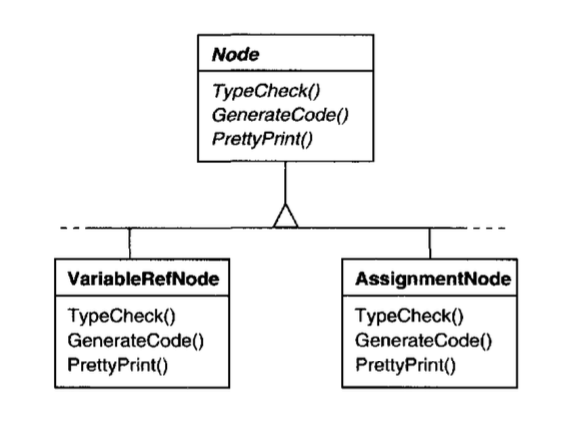
\includegraphics[width=1\linewidth]{assets/pattern/visitor/visitor-esempio-1.png}
    \end{figure}
    \columnbreak
    \begin{figure}[H]
        \centering
        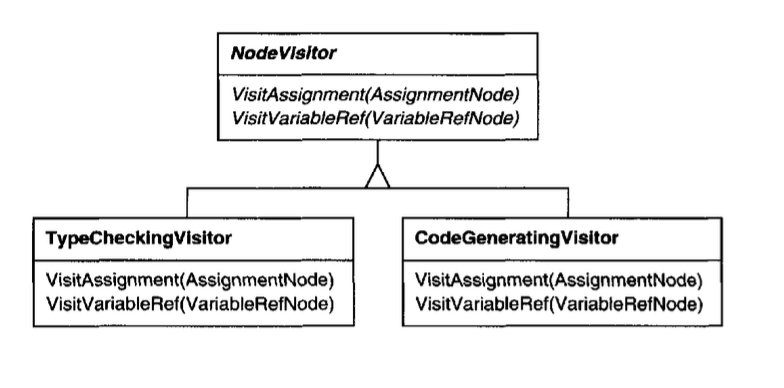
\includegraphics[width=1\linewidth]{assets/pattern/visitor/visitor-esempio-2.png}
    \end{figure}
    \begin{figure}[H]
        \centering
        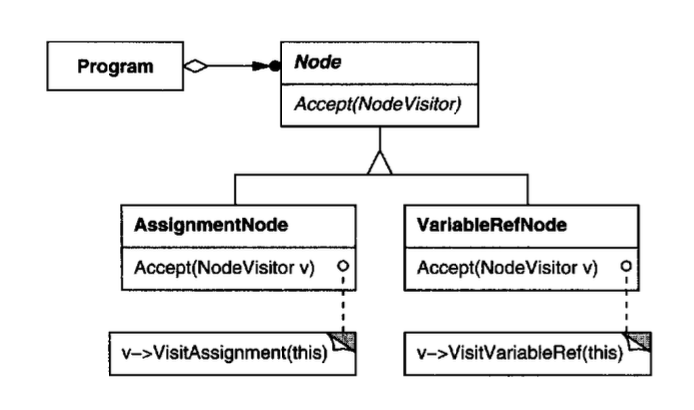
\includegraphics[width=1\linewidth]{assets/pattern/visitor/visitor-esempio-3.png}
    \end{figure}
\end{multicols}

Una soluzione migliore è separare le operazioni dalle classi dei nodi, incapsulandole in oggetti detti visitor, che vengono passati ai nodi durante la traversata dell’AST. Quando un nodo "accetta" un visitor, richiama un metodo specifico del visitor che corrisponde alla sua classe, passando sé stesso come argomento. Ad esempio, per effettuare il type-checking usando i visitor, si crea un oggetto TypeCheckingVisitor e lo si passa all’albero tramite il metodo Accept. I nodi risponderanno chiamando VisitAssignment, VisitVariableReference, ecc. Quello che prima era TypeCheck dentro AssignmentNode diventa VisitAssignment dentro TypeCheckingVisitor. Per supportare più operazioni, si definisce una classe astratta NodeVisitor con un metodo per ogni tipo di nodo. Aggiungere una nuova funzionalità, come il calcolo di metriche, richiederà solo la creazione di una nuova sottoclasse di NodeVisitor, senza modificare le classi dei nodi. Il pattern Visitor permette così di separare in modo pulito la struttura dell’albero (Node hierarchy) dalle operazioni che vi si applicano (Visitor hierarchy), migliorando modularità, estensibilità e manutenibilità del compilatore.

\paragraph{Applicabilità} È consigliabile utilizzare il pattern Visitor quando:
\begin{itemize}
    \item Una struttura di oggetti contiene molte classi di oggetti con interfacce diverse e desideri eseguire operazioni su questi oggetti che dipendono dalle loro classi concrete;
    \item È necessario eseguire molte operazioni distinte e non correlate su oggetti in una struttura di oggetti e desideri evitare di “inquinare” le loro classi con queste operazioni;
    \item Le classi che definiscono la struttura degli oggetti cambiano raramente, ma spesso si desidera definire nuove operazioni sulla struttura;
\end{itemize}

\begin{figure}[H]
    \centering
    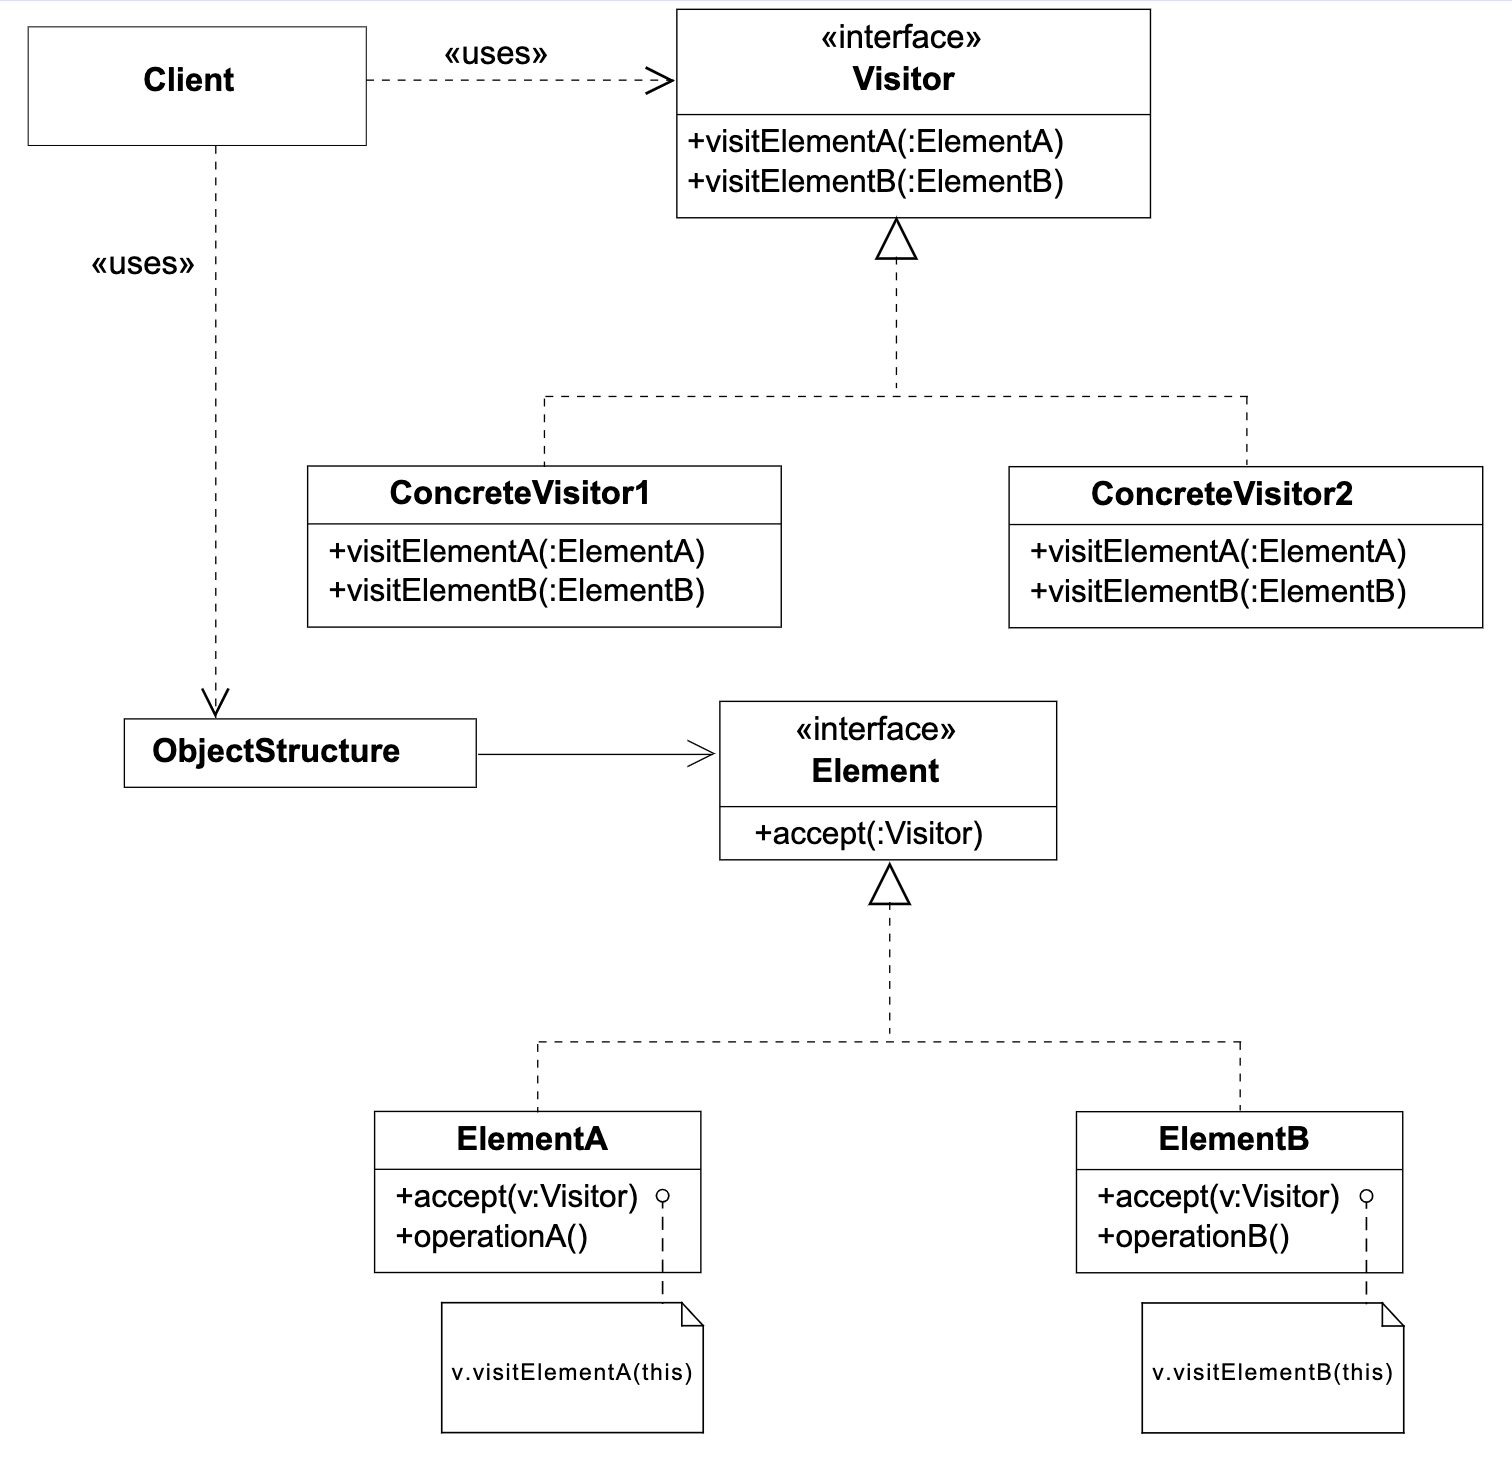
\includegraphics[width=0.75\linewidth]{assets/pattern/visitor/visitor-struttura.png}
    \caption{Class Diagram del pattern Visitor}
\end{figure}

\newpage

\paragraph{Struttura} Il pattern è composto da:
\begin{itemize}
    \item \textbf{Visitor}: dichiara un metodo di visita per ogni classe concreta della struttura, il nome e la firma del metodo identificano la classe che invia la richiesta di visita al visitor in modo che il visitor possa identificare la classe dell’elemento che sta per visitare
    \item \textbf{ConcreteVisitor}: implementa i metodi definiti da Visitor. Ogni metodo implementa un frammento dell’algoritmo definito per la struttura. In più fornisce il contesto per l’algoritmo e memorizza il suo stato locale che accumula durante la visita della struttura.
    \item \textbf{Element}: definisce il metodo \textit{accept()} che riceve un Visitor.
    \item \textbf{ConcreteElements}: implementano il metodo \textit{accept()} che riceve un Visitor.
    \item \textbf{ObjectStructure}: può enumerare gli elementi che la costituiscono. può essere realizzata come un Composite o come una collezione di elementi.
\end{itemize}

\begin{figure}[H]
    \centering
    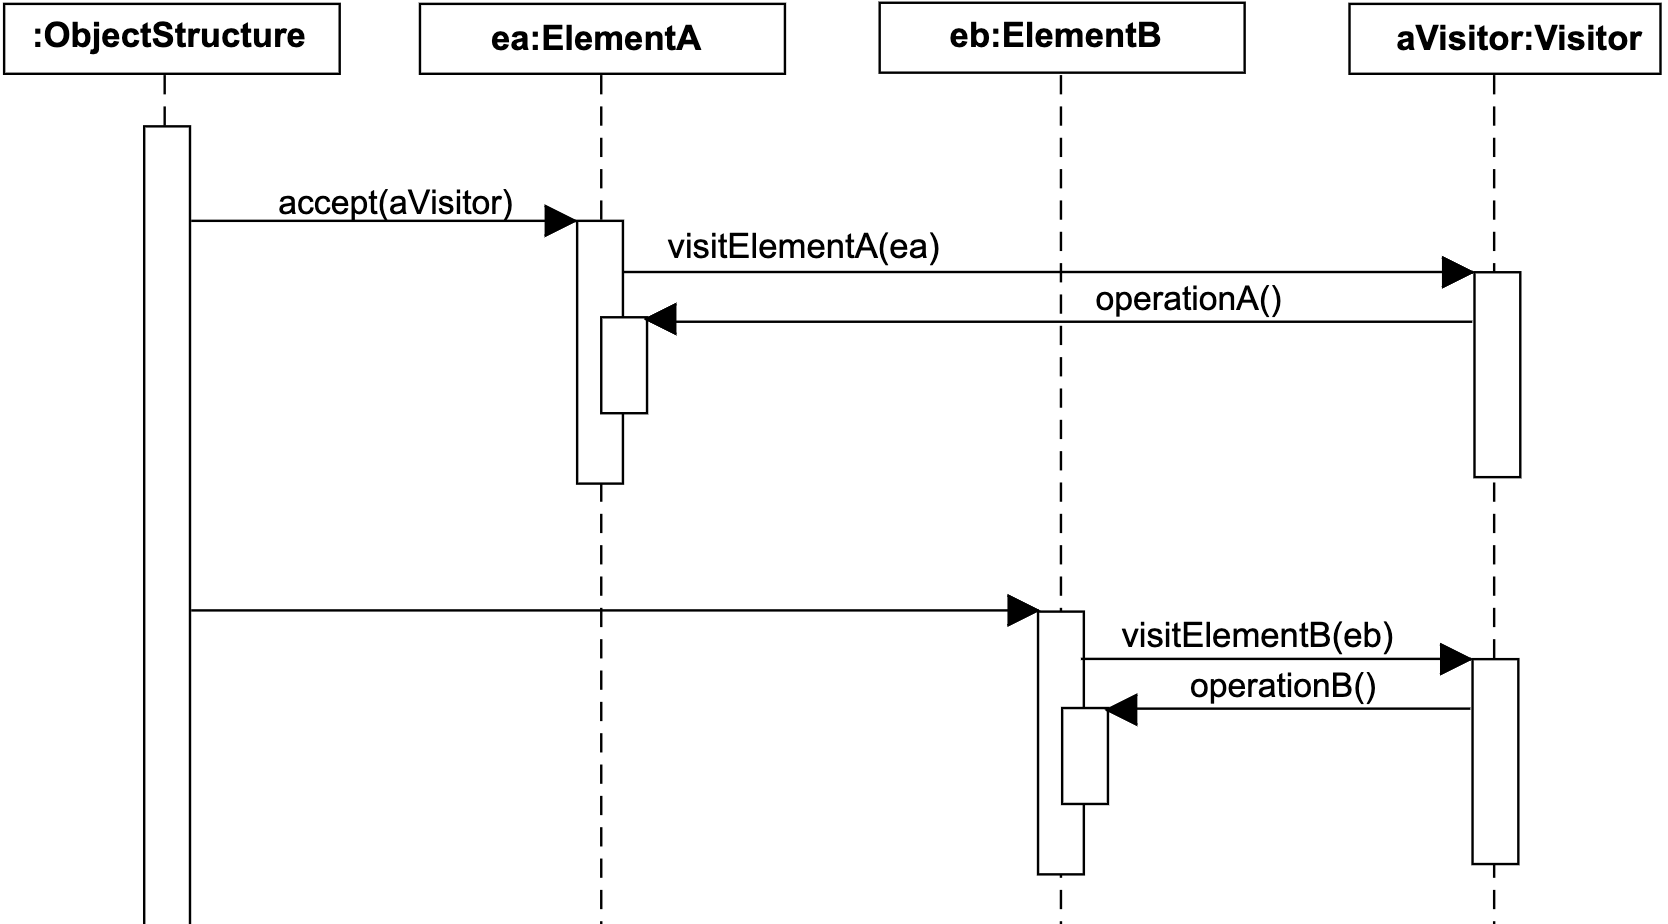
\includegraphics[width=1\linewidth]{assets/pattern/visitor/visitor-sequence.png}
    \caption{Sequence Diagram del pattern Visitor}
\end{figure}

\paragraph{Conseguenze} Il pattern Visitor consente quindi di:
\begin{itemize}
    \item Aggiungere dinamicamente delle nuove operazioni, senza interrompere l'esecuzione: le operazioni vengono integrate in degli oggetti;
    \item Raccogliere le operazioni correlate e separare quelle non correlate;
    \item Visitare gerarchie di classi;
    \item 
\end{itemize}

È bene notare che il pattern rende difficile aggiungere nuove classi ConcreteElement e potrebbe rompere l'incapsulamento (su ConcreteElement).

\paragraph{Pattern correlati} Il pattern Visitor può essere utilizzato per applicare un'operazione su una struttura di oggetti implementata attraverso il pattern Composite (\ref{composite}) oppure per eseguire l'effettiva interpretazione di un'espressione (Interpreter, \ref{interpreter}).


\newpage